\section{Test of the Baseline Algorithm}\label{sec:test_base}
intro
 
\subsection{Alternative to Estimate $\hat{\textbf{A}}$}  
As concluded the Cov-DL algorithm do not recover a sufficient estimate of the mixing matrix $\mathbf{A}$, therefore a different approach is necessary. 

Replacing the insufficient estimate by a fixed estimate $\hat{\mathbf{A}}_{\text{fix}}$ is one immediately solution. 
This choice is supported by the observations from Cov-DL2 where $\mathbf{A}_{\text{ini}}$ matrix provides an estimate which is happens to be a least as good as the one provided by Cov-DL. 
Thus the challenge is now to determine a fixed matrix for which its characteristics resembles those of the true mixing matrix. 
However, from chapter \ref{ch:motivation} it is clear that no specific characteristic of the mixing matrix is known, which supports the choice of an random matrix of Gaussian distribution or similar, as it was chosen for the initial guess $\mathbf{A}_{\text{init}}$ for the estimate.   
From this perspective three fixed mixing matrices are defined, by drawing each entry from a specified distribution: 
\begin{itemize}
\item[] $\hat{\mathbf{A}}_{\text{uni}} \sim \mathcal{U}(-1,1)$
\item[] $\hat{\mathbf{A}}_{\text{norm1}} \sim \mathcal{N}(0,1)$                                           
\item[] $\hat{\mathbf{A}}_{\text{norm2}} \sim \mathcal{N}(0,2)$ 
\end{itemize}
Note that the third matrix $\hat{\mathbf{A}}_{\text{norm1}}$ is generated the same way as the true mixing matrix of the stochastic data sets. 
Thus it is expected to have the lowest MSE when compared to the true mixing matrix $\mathbf{A}$. 
However, it is of interest to investigate whether it is the best estimate of $\mathbf{A}$ which provide the best estimate of $\mathbf{X}$.   

A different option regarding a choice for a fixed $\hat{\mathbf{A}}$ is to utilize the ICA algorithm, described in appendix \ref{app:ICA}. 
By the ICA algorithm it is possible to solve the EEG inverse problem for both $\mathbf{A}$ and $\mathbf{X}$, in the case where $k \leq M$.
Consider a simulation of a stochastic data set specified by $N = k = M$. 
Solving the system by ICA yields an estimate of $\mathbf{A}$. 
Now reduce the data set $\mathbf{Y}$ such that $M \leq k$. 
Similar the estimate of $\mathbf{A}$ is reduced by removing the same rows as in $\mathbf{Y}$, this yields the an estimate $\hat{\mathbf{A}}_{\text{ICA}}$ which can be used as a fixed input to M-SBL along with the corresponding reduced $\mathbf{Y}$.

The four different fixed estimates $\hat{\mathbf{A}}$ are tested on stochastic data sets specified by $M = 10$, $N = k = 16$ and $L = 1000$, where the estimate $\hat{\mathbf{A}}_{\text{ICA}}$ has been reduced to $M = 10$. 
As a reference the $\textbf{A}_{true}$ is included in the plot, to see the best possible $MSE(\textbf{X},\hat{\textbf{X}})$.
To get an average performance 50 different simulations are conducted with the same specifications, each system $\mathbf{X}$ is estimated from each of the four fixed estimates of $\mathbf{A}$\footnote{Note that for each of the 10 repetitions four new $\hat{\mathbf{A}}_{\text{fix}}$ are fixed.}, and the MSE are computed. 
The resulting averaged $\text{MSE}(\mathbf{A}, \hat{\mathbf{A}}_{\text{fix}})$ and $\text{MSE}(\mathbf{X}, \hat{\mathbf{X}})$ are visualised in figure \ref{fig:vary_A}, for each of the four $\hat{\mathbf{A}}_{\text{fix}}$. 
Furthermore, the plotted values are found in table \ref{tab:fixed}.
\begin{figure}[H]
\centering
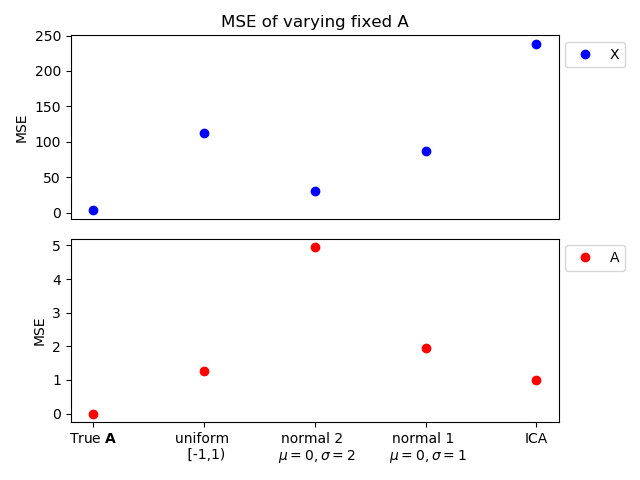
\includegraphics[scale=0.5]{figures/ch_6/A_fix1.png}
\caption{Average MSE values for each of the four fixed mixing matrix $\hat{\mathbf{A}}_{\text{fix}}$ resulting from a stochastic data set specified by $M=10$, $N=k=16$ and $L=1000$.}
\label{fig:vary_A}
\end{figure}
\noindent

\begin{table}[H]
\centering
\begin{tabular}{|c|c|c|c|c|c|}
\hline
 &  $\hat{\mathbf{A}}_{\text{true}}$ & $\hat{\mathbf{A}}_{\text{uni}}$ & $\hat{\mathbf{A}}_{\text{norm2}}$	 & $\hat{\mathbf{A}}_{\text{norm1}}$ & $\hat{\mathbf{A}}_{\text{ICA}}$ \\
\hline
$\text{MSE}(\mathbf{A}, \hat{\mathbf{A}}_{\text{fix}})$ & 0 & 1.271 & 4.957 & 1.941 & 1.006 \\
\hline
$\text{MSE}(\mathbf{X}, \hat{\mathbf{X}})$ & 3.271 & 113.10 & 30.02 & 86.51 & 238.5 \\
\hline
\end{tabular}
\caption{Average MSE values resulting from stochastic data set specified by $M=10$, $N=k=16$ and $L=1000$ with a fixed estimate of the mixing matrix $\hat{\mathbf{A}}_{\text{fix}}$.}
\label{tab:fixed}
\end{table}
\noindent

From table \ref{tab:fixed} and figure \ref{fig:vary_A} it is first of all seen that relation between the MSE of $\textbf{A}$ and $\textbf{X}$ is not as expected, as the lowest $\text{MSE}(\mathbf{A}, \hat{\mathbf{A}}_{\text{fix}})$ results in the highest $\text{MSE}(\mathbf{X}, \hat{\mathbf{X}})$ and so forth. 
The lowest $\text{MSE}(\mathbf{A}, \hat{\mathbf{A}}_{\text{fix}})$ is achieved by using $\hat{\mathbf{A}}_{\text{ICA}}$, which confirms that the ICA algorithm manage to estimate $\mathbf{A}$ when $k \leq M$. 
However, as this do not result in the best estimate of $\mathbf{X}$ a different choice of $\hat{\mathbf{A}}$ is still considered. 
The lowest $\text{MSE}(\mathbf{X}, \hat{\mathbf{X}})$ is achieved by use of $\hat{\mathbf{A}}_{\text{norm}}$, which resulted in the largest $\text{MSE}(\mathbf{A}, \hat{\mathbf{A}}_{\text{fix}})$. 
      
As the main interest in this thesis is to identify and localize the active sources of EEG measurements a low $\text{MSE}(\mathbf{X}, \hat{\mathbf{X}})$ is more desirable than a low $\text{MSE}(\mathbf{A}, \hat{\mathbf{A}}_{\text{fix}})$. 
Furthermore, a disadvantage of using $\hat{\mathbf{A}}_{\text{ICA}}$ is the limitations in practice when $k = M$ is not possible.     
From these observation a fixed estimate of the mixing matrix drawn from a normal distribution with mean 0 and variance 2, $\hat{\mathbf{A}}_{\text{norm}}$, is chosen as the the alternative estimate of $\mathbf{A}$, and is used throughout the thesis. 

Due to the unexpected relation between $MSE(\mathbf{A}, \hat{\mathbf{A}}_{\text{fix}})$ and $\text{MSE}(\mathbf{X}, \hat{\mathbf{X}})$ an additional plot is computed. Figure \ref{fig:X_func_SNR} show the $\text{MSE}(\mathbf{X}, \hat{\mathbf{X}})$ as a function of $\hat{\textbf{A}}$ with varying SNR value. 
Additionally figure \ref{fig:A_func_SNR} show the corresponding MSE between the True $\textbf{A}$ and $\hat{\textbf{A}}$ where an increasing amount of noise is added.
Note that the noise variance is decreasing along the x-axis. 
The noise is generated as Gaussian white noise, with increasing variance corresponding to the desired SNR value. The SNR value is considered in the interval [0.01, 2]. 
From figure \ref{fig:X_func_SNR} it is seen that MSE decreases as the SNR decreases. This indicates as first expected that the better estimate of $\textbf{A}$ the better estimate of $\textbf{X}$. However this is still an contradiction to the result seen in figure \ref{fig:vary_A}. 
This can however be due to the fact that the true $\textbf{A}$ being a Gaussian matrix with $\mu = 0$ and $\sigma = 1$ for which Gaussian noise is added. The MSE between the true $\textbf{A}$ and the noisy $\hat{\textbf{A}}$ seen in figure \ref{fig:A_func_SNR} is not as high as expected due to the relative large amount of noise, all being remarkably less than the corresponding MSE in table \ref{tab:fixed} \todo{det skal tydeliggøres om der er brugt gentagelser her eller er det bare et run. - T}.  


\begin{figure}[H]
    \begin{minipage}[t]{.45\textwidth}
    	\centering
		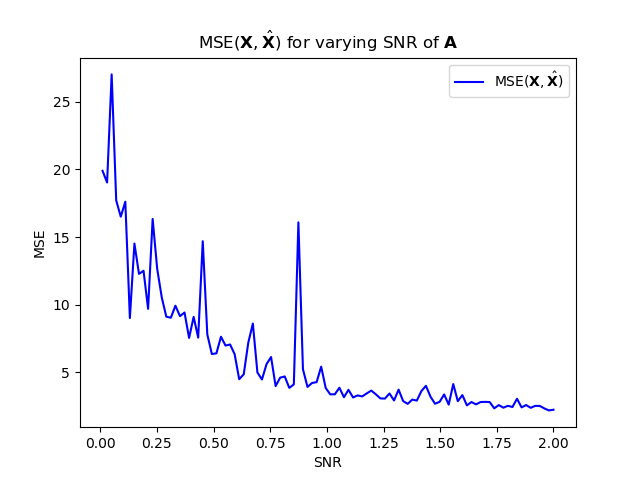
\includegraphics[scale=0.5]{figures/ch_6/X_func_SNR.png}
		\caption{$MSE(\textbf{X},\hat{\textbf{X}})$ estimated from $\textbf{Y}$ specified by $M=6$,$N=k=8$ and $L=1000$, as a function of SNR of given $\textbf{A}$. }
		\label{fig:X_func_SNR}
    \end{minipage} 
    \hfill
    \begin{minipage}[t]{.45\textwidth}
        \centering
		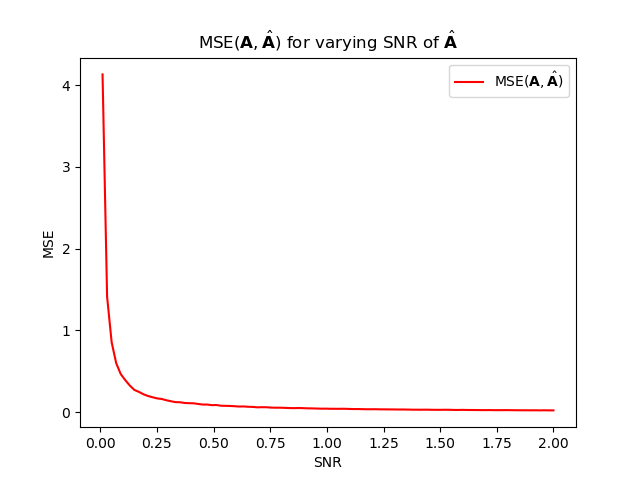
\includegraphics[scale=0.5]{figures/ch_6/A_func_SNR.png}
		\caption{$MSE(\textbf{A},\hat{\textbf{A}})$ where $\hat{\textbf{A}}$ is a function of the SNR. $\hat{\textbf{A}}$ correspond to $\hat{\textbf{A}}$ used in figure \ref{fig:X_func_SNR}}
		\label{fig:A_func_SNR}
    \end{minipage}
\end{figure}  

\subsection{Test}
In order to evaluate the performance of the resulting baseline algorithm tests are conducted on several simulated stochastic data sets with different specification. The aim is to see how the relationship between $N$ and $M$ affect the performance, in other word how robust the algorithm is towards low density measurements. 
The baseline algorithm is on an AR data specified by $M=8$, $L=1000$, $k=N$ and N in the range $N = [M+1, 36]$, as such $k<\frac{M(M+1)}{2}$ are withhold insuring a solution.
For each value of $N$ 5 different data sets are simulated and solved and the average MSE are used as the result. The result are plotted in figure \ref{fig:varyN1}, the MSE is plotted for both $\textbf{X}$ and $\textbf{A}$. 
Due to the performance of COV-DL not being as good as expected, a similar test is made where the true $\textbf{A}$ is given as input to M-SBL. These results are visualised in figure \ref{fig:varyN2}.    
      
\begin{figure}[H]
    \begin{minipage}[t]{.45\textwidth}
    	\centering
		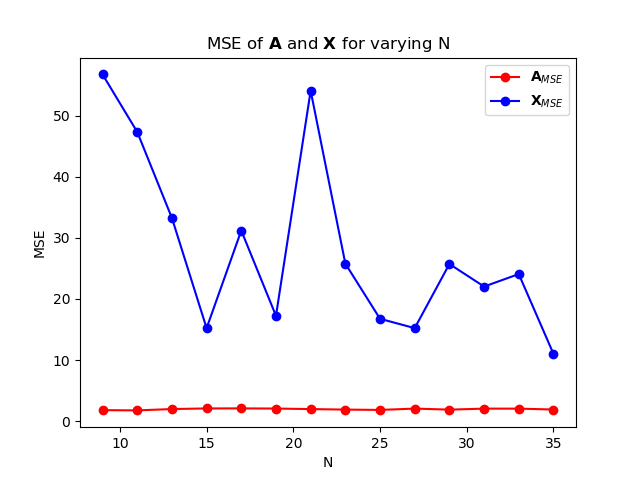
\includegraphics[scale=0.5]{figures/ch_6/varyN_recA.png}
		\caption{ $M = 3$, $k=4$ and $L=1000$}
		\label{fig:varyN1}
    \end{minipage} 
    \hfill
    \begin{minipage}[t]{.45\textwidth}
        \centering
		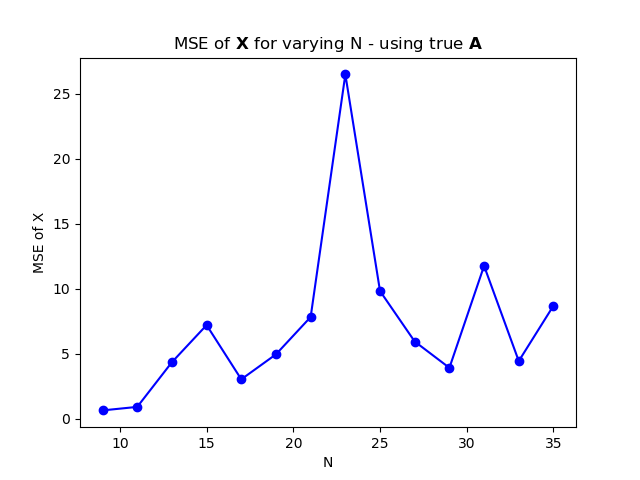
\includegraphics[scale=0.5]{figures/ch_6/varyN_trueA.png}
		\caption{True $\textbf{A}$ $M = 3$, $k=4$ and $L=1000$ }
		\label{fig:varyN2}
    \end{minipage}
\end{figure}

From the results it is seen that .. 



